\chapter{Аналитический раздел}
\label{cha:analysis}

В этом разделе анализируются существующие алгоритмы построения трехмерных изображений
и выбираются наиболее подходящие алгоритмы для решения поставленных задач.

\section{Формализация объектов сцены}


Поскольку это динамическая сцена, время рендеринга кадра должно быть быстрым,
поэтому ограничение - 1 источник света, около 4 сфер, 2 куба.

Сцена состоит из:

\begin{itemize}
  % \item Camera: pinhole camera, has it own coordinate, image plane, can change position
  % \item Light: only one point light, may stay or move on orbit

  \item Камера: пинхол-камера, имеет собственные координаты, плоскость изображения, может изменять положение
  \item Источников света: представляют собой материальную точку,
  представляют собой материальную точку, из которой во всех направлениях исходят лучи света.
  Положение задается трехмерными координатами или запрограммированной орбитой,
  цвет свечения описывается с помощью параметров rgb.
  \item Комната: состоит из 6-ти плоскостей, разных цветов, содержит описание вектор нормали, расстояние до центра сцены
  \item Список сфер: содержит описание положения центра, радиуса, свойств материала.
  \item Список кубов: содержит описание положения центра, длины кромки, свойств материала.
  \item Модель алмаза: полигональная сетка состоит из треугольников.
  \item Материал: $k_a, k_s, k_d, \alpha, ior$
\end{itemize}



\section{Анализ алгоритмов удаления невидимых поверхностей}
% \section{Hidden-surface determination}

При выборе алгоритма определения скрытой поверхности, поскольку это динамическая сцена, нам нужно обратить внимание на то, сколько времени требуется для визуализации кадра, какой алгоритм может хорошо выполнять явления отражения и преломления, и лучше если алгоритм имеет потенциал развития в будущем, способность легко расширяться.

% Известны следующие подходы...


\subsection*{Алгоритм художника}

Алгоритм сортирует все многоугольники в сцене по их глубине, а затем раскрашивает их в этом порядке, от самого дальнего к ближайшему.

При раскрашивании многие пиксели перекрашиваются многократно.
В некоторых случаях алгоритм может давать сбой, включая циклическое перекрытие или пересечение полигонов.
\\
\begin{figure}[ht]
  \centering
  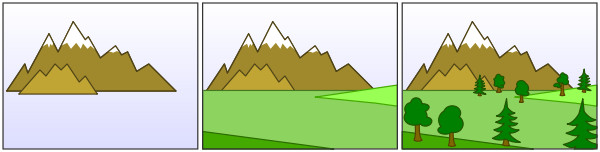
\includegraphics[width=0.8\textwidth]{img/painter.png}
  \caption{Алгоритм художника}
\end{figure}


\subsection*{Алгоритм удаления поверхностей с Z-буфером}

% During rasterization, the depth/Z value of each pixel is checked against an existing depth value. If the current pixel is behind the pixel in the Z buffer, the pixel is rejected, otherwise it is shaded and its depth value replaces that in the B buffer. Z-buffering supports dynamic scenes in a simple way and is currently efficiently implemented in graphics hardware.

Во время растеризации значение глубины (Z) каждого пикселя сравнивается с существующим значением глубины. Если текущий пиксель находится за пикселем в буфере Z, пиксель отклоняется, в противном случае он затеняется, и его значение глубины заменяет значение в буфере. Z-буферизация поддерживает динамические сцены и в настоящее время эффективно реализована в графическом оборудовании.
\\
\begin{figure}[ht]
  \centering
  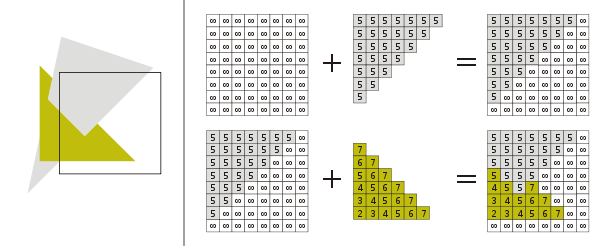
\includegraphics[width=0.8\textwidth]{img/zbuffer.png}
  \caption{Алгоритм Z-буфер}
\end{figure}




\subsection*{Алгоритм Варнока}


Алгоритм работает в пространстве изображения и анализирует область на экране дисплея (окне) на наличие в них видимых элементов. Если в окне нет изображения, то оно просто закрашивается фоном. Если в окне есть элемент, то проверяется, достаточно ли он прост для рендеринга. Если объект сложный, то окно делится на более мелкие, для каждого из которых проводится проверка на отсутствие и/или простоту изображения. Процесс рекурсивного разделения может продолжаться до тех пор, пока не будет достигнут предел разрешения экрана.
\\

Возможны 4 случая взаимного расположения окна и многоугольника:
целиком вне окна, целиком внутри окна, пересекает окно, охватывает окно.



\begin{figure}[ht]
  \centering
  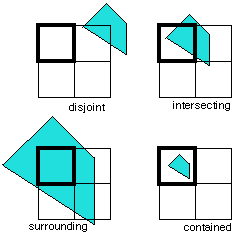
\includegraphics[width=0.35\textwidth]{img/warnock_1.png}
  \hspace{1cm}
  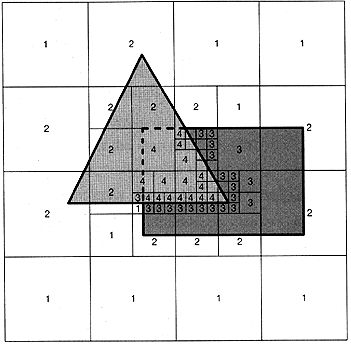
\includegraphics[width=0.35\textwidth]{img/warnock_2.png}
  \caption{Алгоритм Варнока}
\end{figure}


\subsection*{Алгоритм трассировки лучей}


Алгоритм также называется обратной трассировкой лучей, трассировкой пути.

Идея алгоритма заключается в попытке смоделировать путь световых лучей к точке обзора путем прослеживания луча с точки обзора в сцену. Хотя это не алгоритм удаления скрытой поверхности как таковой, он неявно решает проблему удаления скрытой поверхности, находя ближайшую поверхность для каждого видимого луча. Это фактически эквивалентно сортировке всей геометрии по пикселям.

Моделируя световые лучи, мы можем определить, как свет взаимодействует с материалом. Это позволяет нам создавать сцены, похожие на реальность.
Многие физические рендереры разрабатываются на основе этого принципа.

Хорошим моментом является то, что этот алгоритм работает параллельно на графическом процессоре, поскольку каждый пиксель не зависит от других.
Самым большим недостатком этого алгоритма является стоимость вычислений. Чтобы получить более красивое и реалистичное изображение, тем больше время вычислений. За последние несколько лет Nvidia разработала специальные серии графических процессоров для трассировки лучей, некоторые игры начали их поддерживать, поэтому у нее есть возможности для развития в будущем.

\begin{figure}[ht]
  \centering
  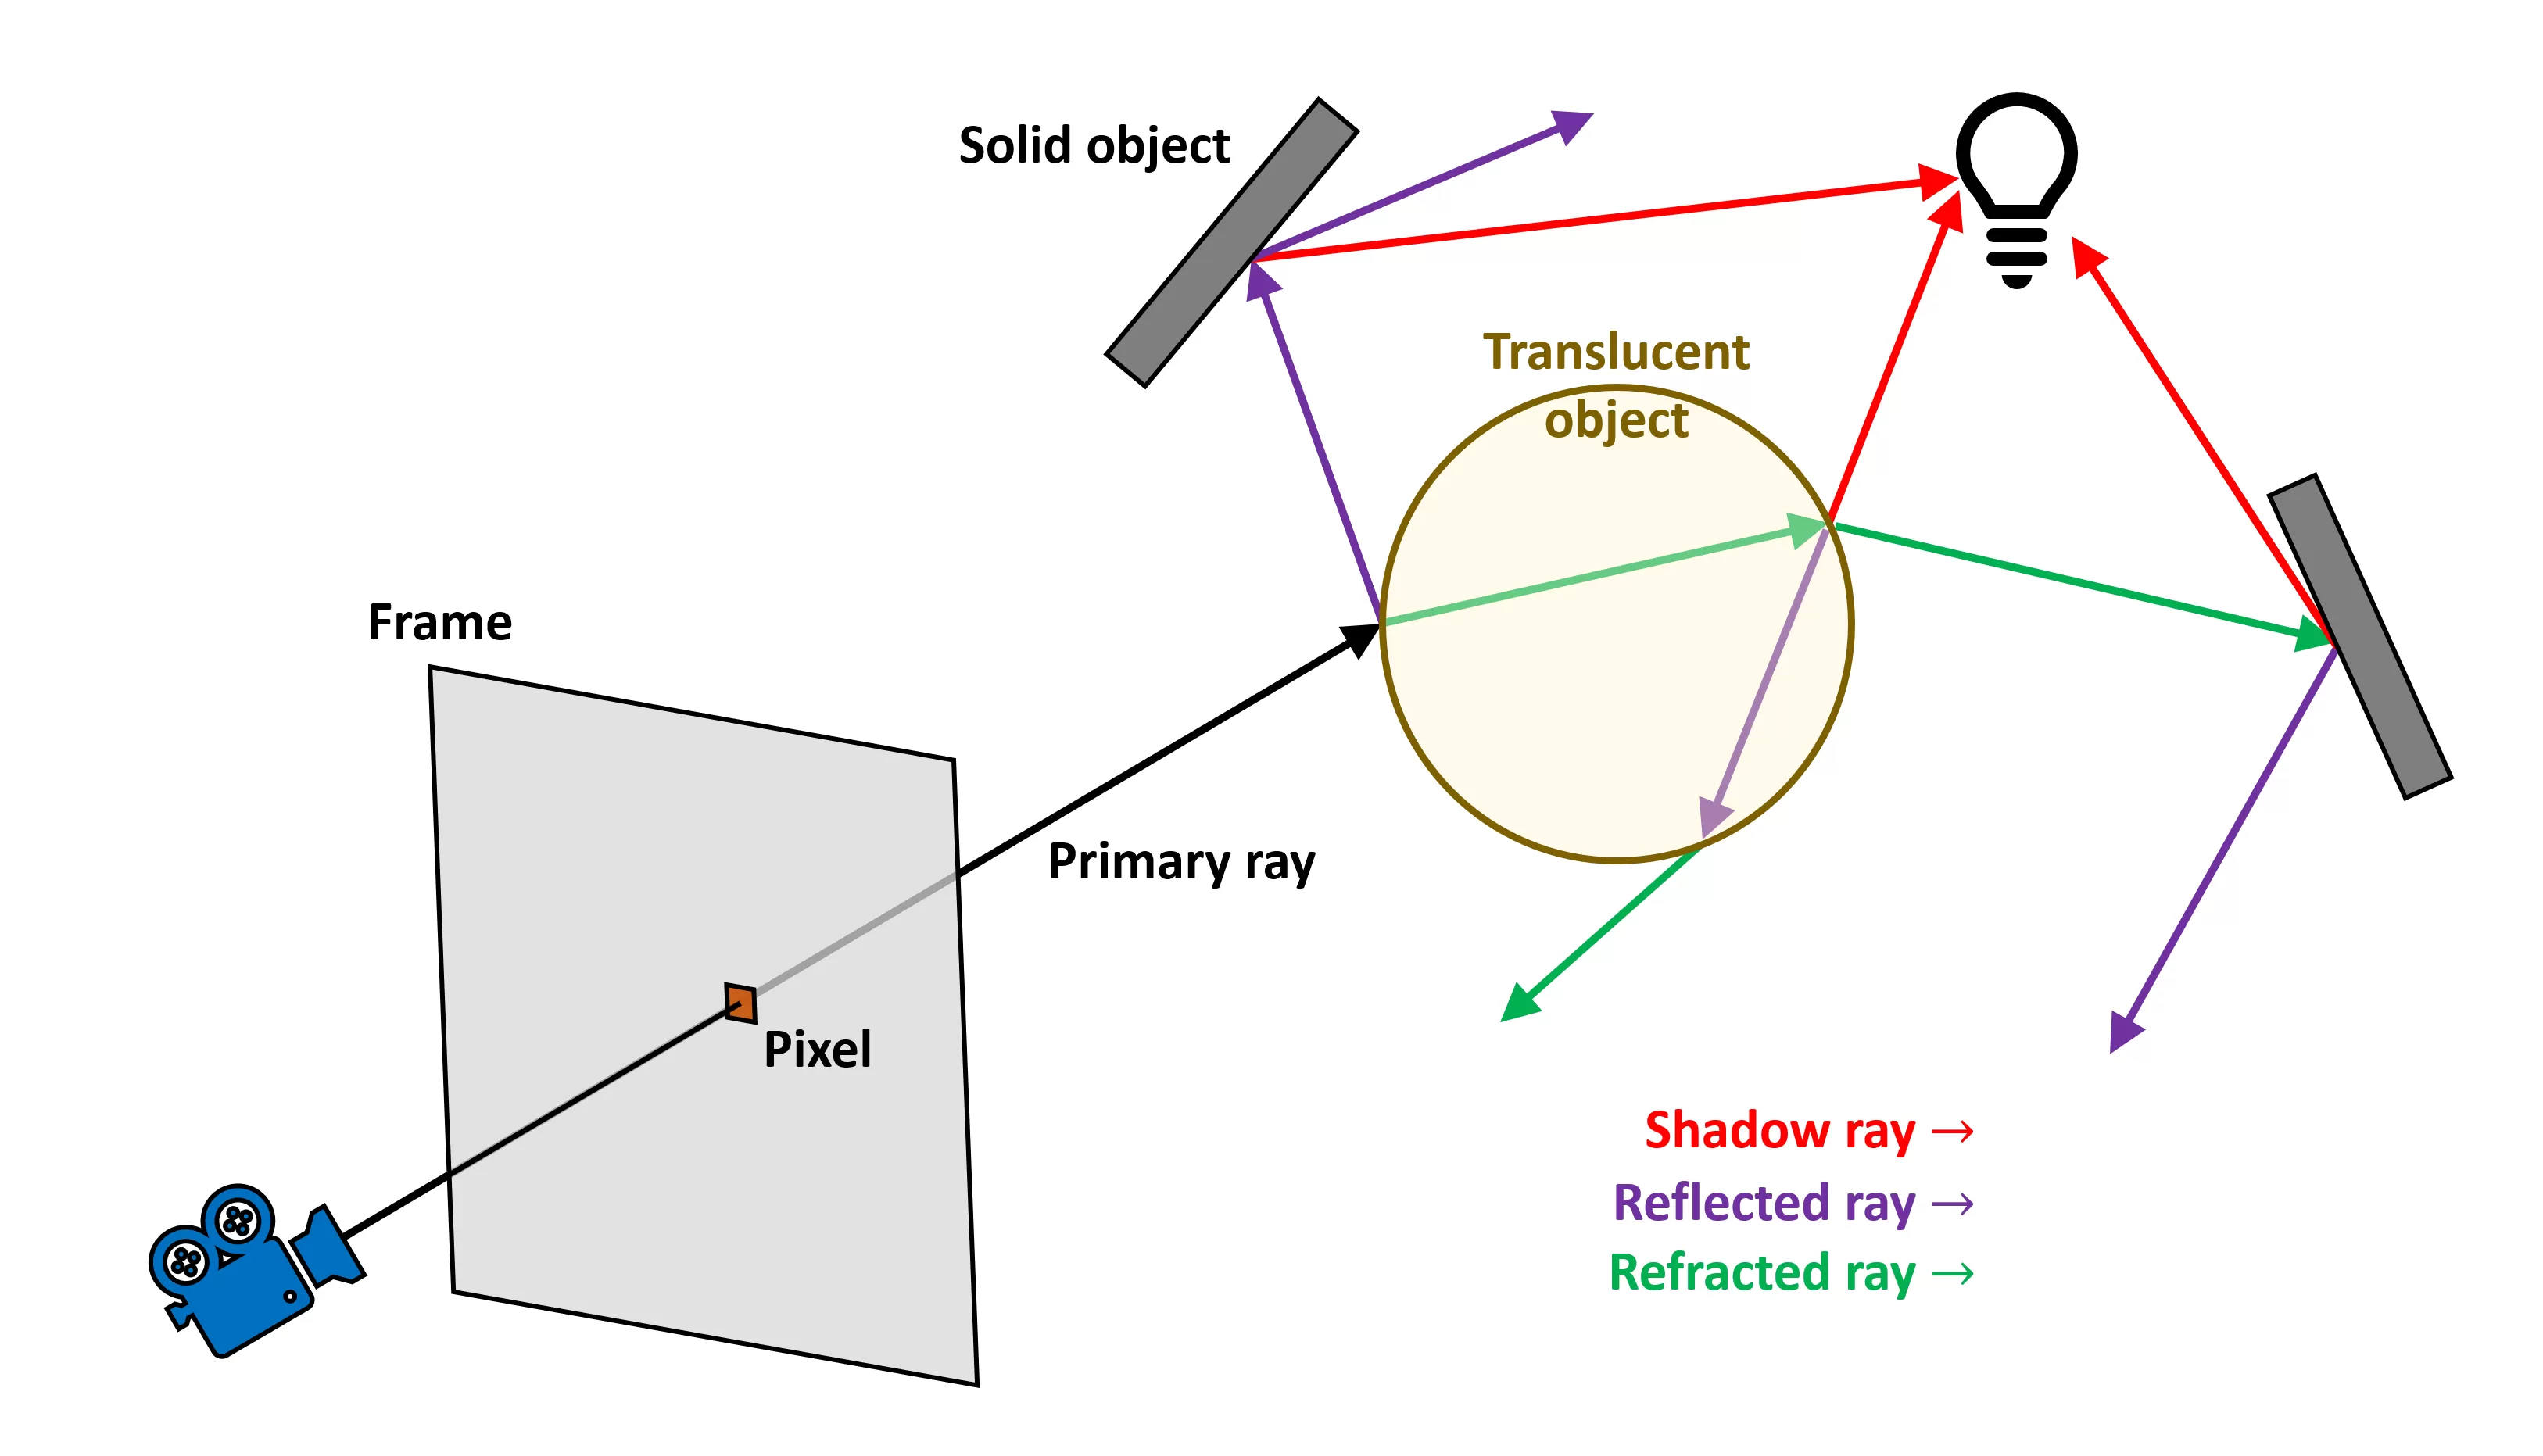
\includegraphics[width=0.8\textwidth]{img/raytracing.png}
  \caption{Алгоритм трассировки лучей}
\end{figure}




\subsection*{Выводы}


% The gpu is designed to run in parallel, so implementing a recursive algorithm is not a good idea, not to mention some famous api graphics like opengl that prohibit recursion.
% Between z-buffer and path tracing i choose algorithm path tracing because it's not too hard, it can show optical phenomena as well as material properties, it can run parallel on gpu for each pixel, it's rapidly growing and widely used.

Алгоритм z-buffer создан для преодоления ограничений алгоритма художника, память, которую он использует, ничтожно мала, поэтому алгоритм z-буфер лучше. Графический процессор разработан для параллельной работы, поэтому реализация рекурсивного алгоритма не является хорошей идеей, не говоря уже о некоторых графических интерфейсах api, таких как opengl, которые запрещают рекурсию, поэтому алгоритм Варнока тоже не подходит.
Между z-буфером и трассировкой лучей я выбираю алгоритм трассировки лучей, потому что это не слишком сложно, он может отображать оптические явления, а также свойства материала, он может работать параллельно на графическом процессоре для каждого пикселя, он быстро растет и широко используется.




\section{Выбор модели освещения}

\subsection*{Модель отражения Фонга}

% Phong reflection is an empirical model of local illumination. It describes the way a surface reflects light as a combination of the diffuse reflection of rough surfaces with the specular reflection of shiny surfaces. The model also includes an ambient term to account for the small amount of light that is scattered about the entire scene.
Отражение Фонга - это эмпирическая модель местного освещения. Он описывает способ отражения света поверхностью как комбинацию диффузного отражения шероховатых поверхностей с зеркальным отражением блестящих поверхностей. Модель также включает в себя окружающий термин для учета небольшого количества света, рассеянного по всей сцене.

Модель отражения Фонга предоставляет уравнение для вычисления освещенности каждой точки поверхности $I_p$
\\

$
{\displaystyle I_p = k_ai_a + \sum_{m\in lights}(k_d(L_m.N)i_{m,d} + k_s(R_m.V)^\alpha i_{m,s})}
$\\\\
где:\\
$k_a, k_s, k_d$ - коэффициент фонового, зеркального, диффузного освещения\\
$i_s, i_d$ - интенсивности зеркальной и диффузной составляющих источника света\\
$i_a$ - интенсивности окружающего света от всех источников света\\
$\alpha$ - которая является константой яркости материала\\
$L$ - вектор направления от точки на поверхности к источнику света\\
$N$ - нормаль в этой точке на поверхности\\
$R$ - направление, в котором идеально отраженный луч света будет направлен из этой точки на поверхности\\
$V$ - направление, указывающее на зрителя.

\begin{figure}[ht]
  \centering
  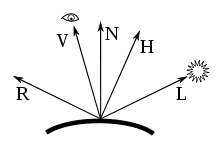
\includegraphics[width=0.4\textwidth]{img/blinn_vectors.png}
  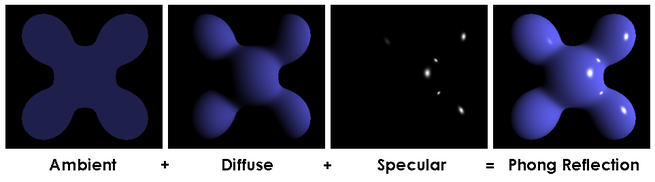
\includegraphics[width=0.8\textwidth]{img/phong_components.png}
  \caption{Модель отражения Фонга}
\end{figure}


\subsection*{Модель отражения Блинна – Фонга}

Модель отражения Блинна является модификацией, разработанной Блинном для модели отражения Фонга.

При затенении Фонга необходимо постоянно пересчитывать скалярное произведение $R.V$ между зрителем (V) и лучом от источника света (L), отраженным (R) от поверхности.
Вычислить средний вектор между векторами наблюдателя и источника света,
\\

$H = \dfrac{L + V}{||L + V||}$\\\\
$R.V$ можно заменить на $N.H$, где $N$ - нормализованная нормаль поверхности.



\subsection*{Преломление}
Когда световые лучи переходят из одной прозрачной среды в другую, они меняют направление. Новое направление луча зависит от двух факторов. Угол падения луча и новый средний показатель преломления или показатель преломления (иногда называемый ior).
Преломление описывается законом Снеллиуса.

\begin{figure}[ht]
  \centering
  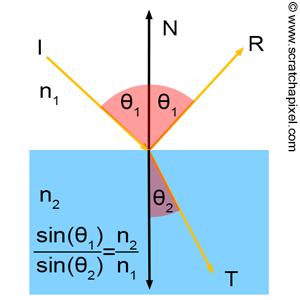
\includegraphics[height=0.3\textwidth, width=0.35\textwidth]{img/refraction.png}
  \caption{Преломление}
\end{figure}


\section{Алгоритм построения теней}

% We cast a shadow ray from the intersection point to the light. If this particular ray does not intersect an object on its way to the light, the hit point is illuminated. If it does intersect with another object, that object casts a shadow on it.
С алгоритмом трассировки лучей тень будет легко рассчитана.
От точки пересечения к свету отбрасываем луч тени. Если этот конкретный луч не пересекает объект на своем пути к свету, точка попадания подсвечивается. Если он пересекается с другим объектом, этот объект отбрасывает на него тень.

\begin{figure}[ht]
  \centering
  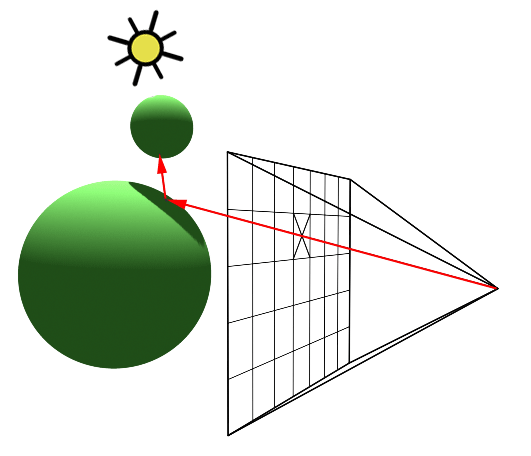
\includegraphics[width=0.4\textwidth]{img/shadow_ray.png}
  \caption{Алгоритм трассировки лучей - тень}
\end{figure}

